\documentclass[letterpaper]{article}
\usepackage{aaai}
\usepackage{times}
\usepackage{helvet}
\usepackage{courier}
\usepackage{amsmath, amssymb}
\usepackage{graphicx}
\usepackage{booktabs}
\usepackage{algorithm}
\usepackage{algorithmic}
\usepackage{multirow}
\usepackage{url}
\frenchspacing
\setlength{\pdfpagewidth}{8.5in}
\setlength{\pdfpageheight}{11in}
\pdfinfo{
/Title (Comparing Function Approximation Methods and State Representations for Reinforcement Learning in Snake)
/Author (Kiran Sairam Bethi Balagangadaran)
/Keywords (reinforcement learning, function approximation, tile coding, Double DQN, state representation)
}
\setcounter{secnumdepth}{0}

\begin{document}

\title{Comparing Function Approximation Methods and State Representations for Reinforcement Learning in Snake}
\author{
Kiran Sairam Bethi Balagangadaran\\
Khoury College of Computer Sciences\\
Northeastern University\\
bethi.k@northeastern.edu
}
\maketitle

\begin{abstract}
\begin{quote}
This project compares three function approximation methods on the game Snake to see how each one handles different state representations. The methods are hand-crafted linear features, hash-based tile coding, and a Double DQN neural network with experience replay. We test each one against three representations of increasing complexity (11, 109, and 126 dimensions), training for 20,000 episodes across 5 random seeds. The neural network performs best on every representation. Its highest score is 29.05 on extended features, which beats our hand-coded greedy heuristic baseline (22.89). Tile coding does well on compact features (22.69) but breaks down at higher dimensions (3.21 on local, 1.32 on extended) because of hash collisions. Linear function approximation learns to avoid danger but never picks up food-seeking, scoring below 4.0 on every representation. Overall, the function approximation method and the representation interact strongly: tile coding works well for low-dimensional, well-designed features, while neural networks generalize across all representations when stabilized by Double DQN and experience replay.
\end{quote}
\end{abstract}

\section{Introduction}

Reinforcement learning (RL) has done well on game-playing domains, from TD-Gammon's near-expert backgammon play \cite{tesauro1995tdgammon} to DQN's human-level Atari performance \cite{mnih2015dqn}. One recurring question across these results is how state representation and function approximation interact: how the state is represented and how the value function is approximated together decide whether an agent can learn at all.

The two extremes of this question are well studied (tabular methods on small state spaces, deep neural networks on raw pixel inputs), but the middle ground is less clear. When is a simple linear model enough? When does automatic feature construction (tile coding) beat hand-crafted features? At what point do you actually need a neural network? These questions matter for problems where deep RL is overkill but tabular methods are too small.

We use the classic game Snake to study these questions. Snake is a good test case because it offers a natural range of state representations: from a small 11-dimensional binary feature vector (danger signals and food direction) to a 126-dimensional vector that combines a local grid window with continuous distance features. The game also gets harder within an episode as the snake grows, so the effective state space is non-stationary, which puts pressure on every method.

Our contributions are as follows. First, we compare three function approximation methods (hand-crafted linear features, hash-based tile coding, and a Double DQN neural network with experience replay) across three state representations using the same experimental setup. Second, we show that tile coding beats hand-crafted linear features by a large margin on the compact representation ($22.69$ vs.\ $0.80$), which highlights the value of automatic feature construction. Third, we show that Double DQN with experience replay gets the highest score overall ($29.05$ on extended features), beats the greedy heuristic by 27\%, and keeps low variance across all three representations. Fourth, we show that the function approximation method and the representation interact strongly: tile coding gets worse as dimensionality goes up, while neural networks do not.

\section{Background}

\subsection{Temporal-Difference Learning}

Temporal-difference (TD) learning \cite{sutton1988td} updates value estimates from the difference between successive predictions, without waiting for the episode to end. For control, SARSA \cite{rummery1994sarsa} updates the action-value function from the transition $(S_t, A_t, R_{t+1}, S_{t+1}, A_{t+1})$:
\begin{multline}
    Q(S_t, A_t) \leftarrow Q(S_t, A_t) + \\
    \alpha \left[ R_{t+1} + \gamma Q(S_{t+1}, A_{t+1}) - Q(S_t, A_t) \right]
\end{multline}
where $\alpha$ is the learning rate and $\gamma$ is the discount factor. SARSA is on-policy: it evaluates and improves the policy currently being followed, including its exploratory actions.

\subsection{Function Approximation}

When the state space is too large for tabular methods, the value function has to be approximated. In \textbf{linear function approximation}, the action-value function is:
\begin{equation}
    \hat{q}(s, a; \mathbf{w}) = \mathbf{w}^\top \mathbf{x}(s, a)
\end{equation}
where $\mathbf{x}(s, a) \in \mathbb{R}^d$ is a feature vector and $\mathbf{w} \in \mathbb{R}^d$ is a weight vector. The semi-gradient SARSA update becomes:
\begin{equation}
    \mathbf{w} \leftarrow \mathbf{w} + \alpha \delta_t \, \mathbf{x}(S_t, A_t)
    \label{eq:linear_update}
\end{equation}
where $\delta_t = R_{t+1} + \gamma \hat{q}(S_{t+1}, A_{t+1}; \mathbf{w}) - \hat{q}(S_t, A_t; \mathbf{w})$.

\textbf{Tile coding} \cite{sutton2018reinforcement,sherstov2005tilecoding} builds binary feature vectors automatically. Multiple overlapping tilings split up the normalized state space, and the feature vector has one active bit per tiling. The value function is the sum of weights at the active tile indices. Nearby states share most of their active tiles, which gives smooth generalization.

\textbf{Neural network approximation} replaces the linear model with a nonlinear function parameterized by $\boldsymbol{\theta}$, updated using backpropagation. \textbf{Double DQN} \cite{vanhasselt2016deep} fixes the overestimation bias in vanilla DQN by separating action selection from action evaluation: the online network picks the greedy next action $\hat{a} = \arg\max_a Q(S_{t+1}, a; \boldsymbol{\theta})$, while a periodically-synchronized target network scores it:
\begin{equation}
    Y_t = R_{t+1} + \gamma Q(S_{t+1}, \hat{a}; \boldsymbol{\theta}^-)
\end{equation}
Combined with a replay buffer that breaks up the temporal correlations in the training data, this stabilizes learning with nonlinear function approximation.

\subsection{The Deadly Triad}

Sutton and Barto \shortcite{sutton2018reinforcement} call out the \emph{deadly triad}: function approximation, bootstrapping, and off-policy learning together can cause divergence. Tsitsiklis and Van Roy \shortcite{tsitsiklis1997analysis} proved that on-policy TD with linear function approximation converges with probability 1, while Baird \shortcite{baird1995residual} showed that off-policy TD with linear FA can diverge even in simple cases. Van Hasselt et al.\ \shortcite{vanhasselt2018deadly} showed that these risks are real in deep RL settings too.

Our linear and tile coding agents use on-policy semi-gradient SARSA, so they keep the convergence guarantee. Our neural network agent breaks the on-policy assumption by using experience replay, which puts it on the off-policy side of the deadly triad. We deal with this using Double DQN (to reduce overestimation bias) and a hard-synchronized target network (to keep the regression target stable), which is standard practice in deep RL \cite{mnih2015dqn,vanhasselt2016deep}.

\section{Related Work}

\subsection{Snake as an RL Domain}

Snake has been studied with a range of RL methods. Wei et al.\ \shortcite{wei2018autonomous} used DQN with a CNN over raw pixel frames and added dual experience replay and a training gap strategy. Bonnici et al.\ \shortcite{bonnici2022exploring} compared Q-learning, SARSA, PPO, and A* across vector, CNN, and raycasting representations, and found that PPO with raycasting did best. Sebastianelli et al.\ \shortcite{sebastianelli2021deep} showed that a sensor-based 11-value state representation trains much more easily than a CNN approach. A Stanford CS230 project by Jiang and Mai compared an 11-boolean feature vector against grayscale screenshots and found that the compact features got sevenfold higher scores \cite{jiang2021snakeai}. Ma et al.\ \shortcite{ma2016snake} found that SARSA outperformed Q-learning on Snake with 128 discrete states, and proved that optimal Snake play involves NP-hard subproblems.

\subsection{Linear FA vs.\ Neural Networks}

Liang et al.\ \shortcite{liang2016shallow} showed that hand-crafted features with linear function approximation can match DQN performance on Atari games. Elfwing et al.\ \shortcite{elfwing2018sigmoid} compared TD($\lambda$) with neural networks against linear FA on Tetris, and found that neural networks did much better when the value function was inherently nonlinear. Tesauro \shortcite{tesauro1995tdgammon} showed that adding hand-crafted expert features to a neural network gave a big improvement to TD-Gammon's performance.

\subsection{Positioning}

We aren't aware of prior work that systematically compares all three of these function approximation methods (hand-crafted linear features, tile coding, and a neural network) across multiple state representations for Snake using a common framework. Most existing studies use off-policy DQN and focus on the neural network side. We try to fill that gap by holding the training framework fixed and varying both the approximation method and the representation.

\section{Methods}

\subsection{Environment}

We implement a custom Snake environment on a $20 \times 20$ grid using the Gymnasium interface \cite{gymnasium}. The snake starts at the center with length 3, facing right. The action space is $\mathcal{A} = \{\text{STRAIGHT}, \text{LEFT}, \text{RIGHT}\}$ relative to the current heading, which removes the option of reversing into the snake's body. Rewards are $+10$ for eating food, $-10$ for dying (wall or self-collision), and $-0.1$ per step to encourage efficiency. The discount factor is $\gamma = 0.95$. Episodes terminate on death or after $3 \times \text{grid\_size}^2 = 1{,}200$ steps (truncation).

For the neural network agent, we add potential-based reward shaping \cite{ng1999reward}: a bonus of $F(s, s') = 0.5 \times (d(s) - d(s'))$ is added at each step, where $d$ is the Manhattan distance from the snake's head to the food. The bonus is skipped on the step where food is eaten, since the food position resets and the comparison would be meaningless. Potential-based shaping does not change the optimal policy \cite{ng1999reward}, but it gives a denser reward signal that speeds up learning.

\subsection{State Representations}

We compare three representations of increasing complexity.

\textbf{Compact (11 dimensions):} Three binary danger signals (wall or body one step ahead in each relative direction), four one-hot direction bits, and four binary food-direction indicators. This matches the standard design used in most Snake RL implementations \cite{loeber2020snakeai,zhou2023snake}.

\textbf{Local Neighborhood (109 dimensions):} A $5 \times 5$ grid window centered on the snake's head, with each cell one-hot encoded as [empty, food, wall, body] (100 features), plus food direction (4) and a snake length bucket (5).

\textbf{Extended (126 dimensions):} The local neighborhood features plus the normalized Manhattan distance to food (1), the distance to the nearest body segment in each cardinal direction (4), the distance to walls (4), the normalized snake length (1), the current direction one-hot (4), and explicit danger signals (3).

For the linear and tile coding models, we build state-action features by one-hot action stacking: the state vector is placed in the block corresponding to the action and zero elsewhere, which gives feature dimensions of 33, 327, and 378 respectively.

\subsection{Algorithms}

All three algorithms use $\varepsilon$-greedy exploration with $\varepsilon$ decaying linearly from 1.0 to 0.01 over 80\% of the 20,000 training episodes.

\textbf{Linear FA SARSA.} The update is Equation~\ref{eq:linear_update} with learning rate $\alpha = 0.01$.

\textbf{Tile Coding SARSA.} We use overlapping tilings with 4 tiles per dimension and a hash table with 262,144 entries. We use 8 tilings for the compact representation and 4 tilings for local and extended (more tilings give diminishing returns once the hash table is fixed at 262k). The effective learning rate is $\alpha = 0.05 / n_{\text{tilings}}$, following the standard convention \cite{sutton2018reinforcement}. Feature normalization ranges are estimated by sampling 1,000 random episodes before training.

\textbf{Double DQN.} A two-layer network with hidden dimensions (256, 128) and ReLU activations outputs Q-values for all three actions at once. We use a replay buffer of capacity 50,000, and sample mini-batches of 64 transitions per gradient step. The target network is hard-copied from the online network every 100 episodes. The training target is the Double DQN target described in the Background section: the online network picks the greedy next action and the target network scores it, which reduces overestimation bias. The loss is Huber (smooth $\ell_1$) for robustness to large TD errors. We use the Adam optimizer \cite{kingma2015adam} with learning rate $10^{-3}$ and gradient clipping at max norm 5.0. Distance-based reward shaping is applied during training.

\subsection{Baselines}

We compare against two baselines: a \textbf{random policy} (uniform random actions) and a \textbf{greedy heuristic} that avoids immediate danger and moves toward food by Manhattan distance.

\section{Experiments}

\subsection{Experimental Setup}

We run 9 configurations (3 algorithms $\times$ 3 representations), each for 20,000 episodes across 5 random seeds. Performance is measured as the average score (food eaten per episode) over the final 1,000 episodes. We report mean and standard deviation across seeds. Learning curves are smoothed with a 100-episode moving average.

\subsection{Tabular Methods Break Down}

To motivate function approximation, we first run tabular Q-learning on all three representations using a smaller $10 \times 10$ grid (3,000 episodes). Table~\ref{tab:tabular} shows the results.

\begin{table}[t]
\centering
\small
\caption{Tabular Q-learning on a 10$\times$10 grid (3,000 episodes). Richer representations cause state space explosion.}
\label{tab:tabular}
\begin{tabular}{lcrrr}
\toprule
Representation & Dims & States & Q-entries & Score \\
\midrule
Compact        & 11   & 253        & 694    & 9.00 \\
Local          & 109  & 7,443      & 13,649 & 1.93 \\
Extended       & 126  & 28,160     & 41,909 & 0.40 \\
\bottomrule
\end{tabular}
\end{table}

The compact representation has only 253 unique states and gets a strong score (9.00). The local neighborhood produces 7,443 unique states (most visited only once), and the score drops to 1.93. The extended representation explodes to 28,160 unique states with near-random performance (0.40 vs.\ 0.15 for a random policy). This confirms that function approximation is needed for the richer representations.

\subsection{Baseline Performance}

On the $20 \times 20$ grid (200 evaluation episodes), the random policy scores $0.15 \pm 0.38$ (max 2), dying mostly from wall collisions. The greedy heuristic scores $22.89 \pm 6.00$ (max 33), dying mostly from self-collision because it chases food without planning around its own body. These give us lower and upper reference points.

\subsection{Main Results}

Table~\ref{tab:main_results} shows the final performance across all 9 configurations after 20,000 training episodes.

\begin{table}[t]
\centering
\small
\caption{Final performance (mean $\pm$ std over the last 1,000 episodes, 5 seeds) on a 20$\times$20 grid after 20,000 training episodes. Bold marks the best score per column.}
\label{tab:main_results}
\begin{tabular}{lccc}
\toprule
 & \textbf{Compact} & \textbf{Local} & \textbf{Extended} \\
\midrule
Linear FA   & $0.80 \pm 0.07$           & $0.67 \pm 0.03$           & $3.90 \pm 0.98$ \\
Tile Coding & $22.69 \pm 0.54$          & $3.21 \pm 0.17$           & $1.32 \pm 0.03$ \\
Double DQN  & $\mathbf{24.26 \pm 0.39}$ & $\mathbf{22.51 \pm 0.38}$ & $\mathbf{29.05 \pm 0.32}$ \\
\bottomrule
\end{tabular}
\end{table}

\begin{figure}[t]
\centering
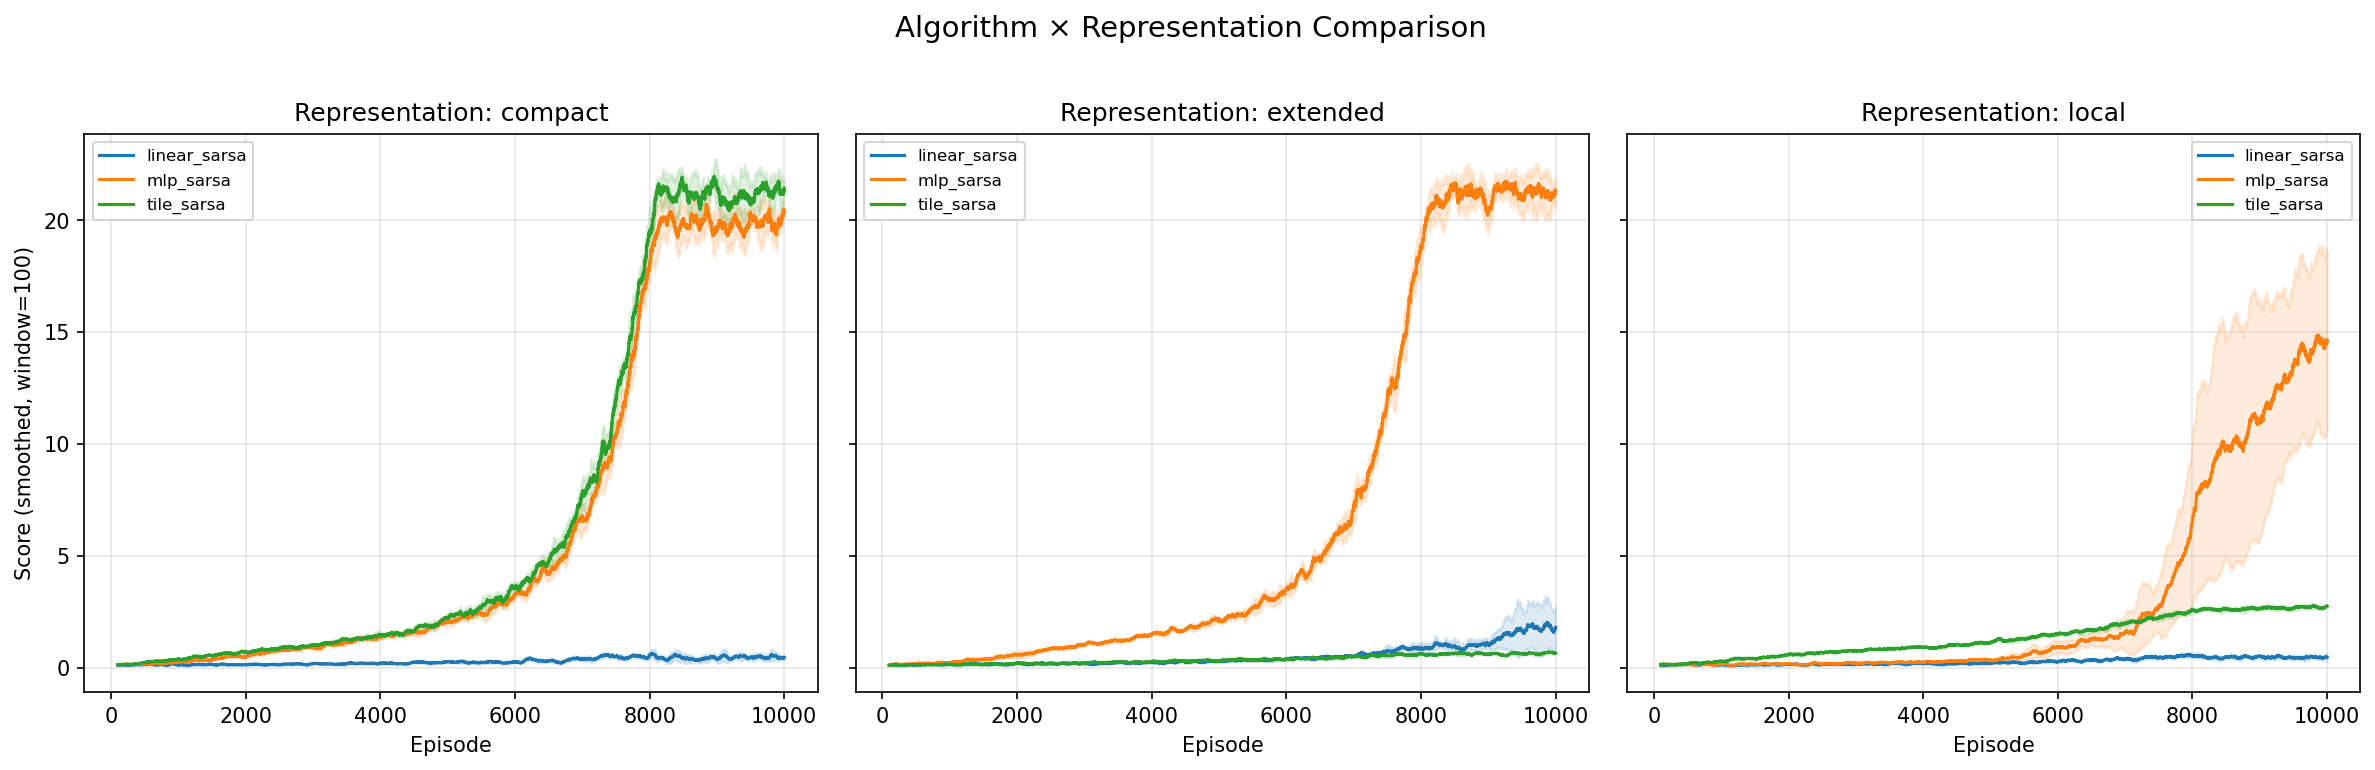
\includegraphics[width=\columnwidth]{comparison_by_representation.png}
\caption{Learning curves across all 9 configurations grouped by representation. Shaded regions show $\pm 1$ std across 5 seeds.}
\label{fig:learning_curves}
\end{figure}

\begin{figure}[t]
\centering
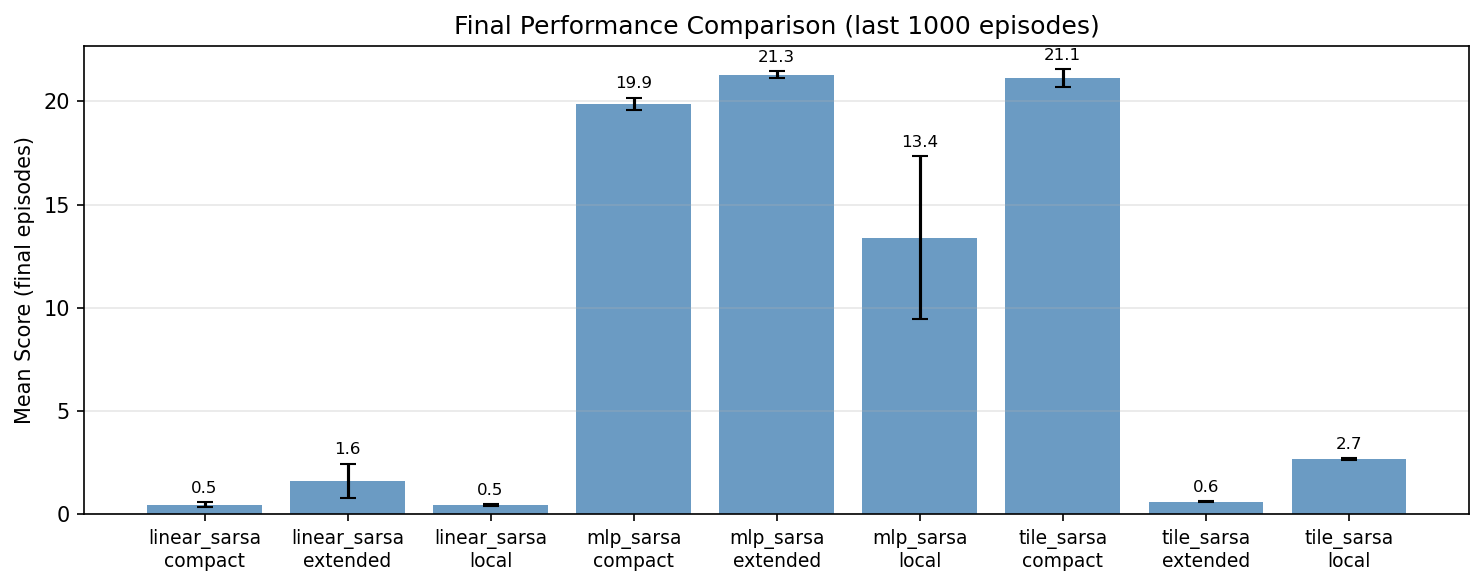
\includegraphics[width=\columnwidth]{final_performance.png}
\caption{Final performance bar chart across all configurations, grouped by representation.}
\label{fig:final_perf}
\end{figure}

\begin{figure}[t]
\centering
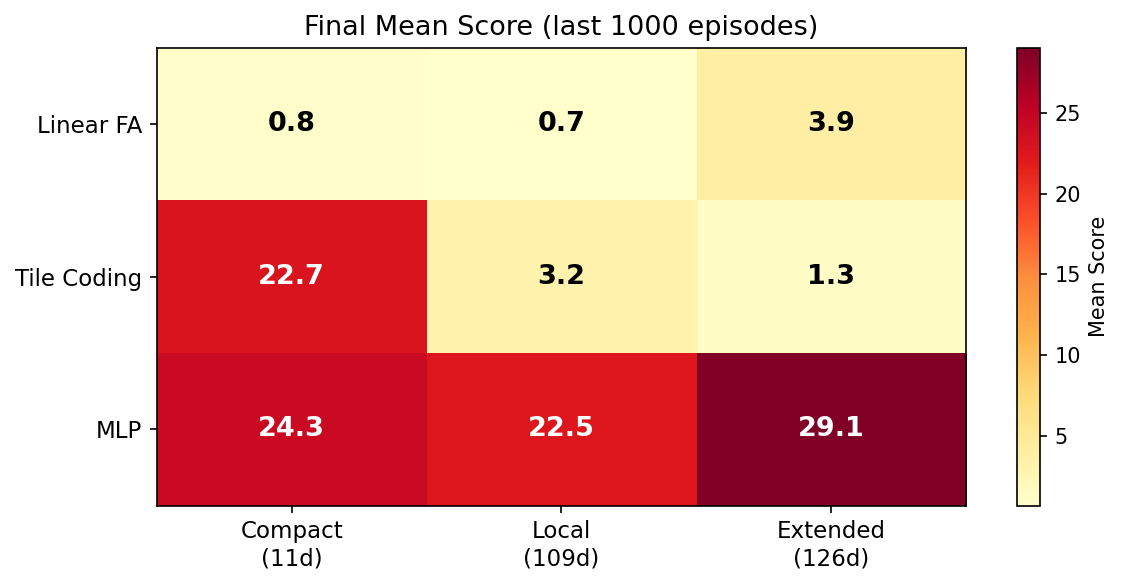
\includegraphics[width=\columnwidth]{heatmap.png}
\caption{3$\times$3 heatmap of mean scores over the final 1,000 episodes (algorithms $\times$ representations). Double DQN dominates all cells; tile coding is competitive only on compact.}
\label{fig:heatmap}
\end{figure}

\subsection{Analysis}

\subsubsection{Representation and Approximation Interaction.}

The results show a strong interaction between representation complexity and approximation method, summarized in Figure~\ref{fig:heatmap}. Tile coding does best on compact features (22.69), close to the greedy heuristic (22.89), but drops to 3.21 on local and 1.32 on extended. Double DQN does the opposite: it gets its highest score on extended features (29.05), beating the greedy heuristic by 27\%, and it wins on every representation (24.26 compact, 22.51 local), including beating tile coding on compact (22.69) where tile coding is at its strongest. Linear FA is weak across the board, with a peak of 3.90 on extended.

This pattern is also visible directly in the learning curves (Figure~\ref{fig:learning_curves}) and the bar chart (Figure~\ref{fig:final_perf}). Tile coding generalizes through overlapping tilings, which works well in low dimensions but breaks down once hash collisions become frequent. Neural networks learn how to generalize directly from gradient descent, so they are less tied to a specific representation as long as training is stable and runs long enough.

\subsubsection{Tile Coding vs.\ Hand-Crafted Features.}

Tile coding does $28\times$ better than hand-crafted linear features on the compact representation ($22.69$ vs.\ $0.80$). The reason is that tile coding's overlapping tilings give a much richer feature space than the 33-weight linear model. Nearby states share most of their active tiles, so the value function generalizes smoothly, which the binary features cannot do on their own.

The advantage disappears at higher dimensions. With 109 or 126 input dimensions, the hash-based tile coder maps an enormous index space into 262,144 buckets, and hash collisions become frequent. Genuinely different states end up activating the same tile indices, which corrupts the value function. The drop is monotonic: $22.69 \to 3.21 \to 1.32$, which is a $17\times$ reduction from compact to extended. This is a known limitation of hash-based tile coding \cite{sherstov2005tilecoding}, and it suggests that any use of hash-based linear approximation in a high-dimensional grid world needs some form of dimensionality reduction or feature embedding first.

\subsubsection{Double DQN Stability Across Representations.}

Double DQN has very low variance across all three representations: $\pm 0.39$, $\pm 0.38$, and $\pm 0.32$ on compact, local, and extended. This is no accident. Experience replay breaks up the temporal correlations that make on-policy updates noisy, which gives a more stationary regression problem. Double DQN's decoupled target avoids the overestimation feedback loop that destabilizes vanilla DQN. The target network, hard-copied every 100 episodes, holds the regression target fixed within each update window, which stops value estimates from running away.

Because of this, Double DQN works reliably even on the local representation (22.51), which is high-dimensional and sparse — usually a hard case for on-policy nonlinear approximation \cite{vanhasselt2018deadly}. This suggests that for neural network function approximation in game environments, off-policy infrastructure (replay + target network) is what makes learning consistent.

\subsubsection{Weight Analysis for Linear FA.}

The linear model's weights on the compact representation are easy to interpret. The largest weights are the danger signals: the weight for ``danger straight'' in the STRAIGHT action block reaches roughly $-8$, and the danger weights in the LEFT and RIGHT blocks follow the same pattern. The agent has clearly learned a strong collision-avoidance policy.

The food-direction weights are much smaller and noisier (typically less than 2 in magnitude). The linear model over 11 binary features can express avoidance, but not the kind of food-seeking that needs more nuance. Under a near-greedy policy ($\varepsilon \approx 0.01$), the agent ends up in deterministic loops, because the compact representation maps many distinct game states to the same feature vector and that creates action cycles.

\subsubsection{Qualitative Behavior.}

The clearest contrast is between tile coding and linear FA on the compact representation. The tile coding agent moves toward food efficiently, makes deliberate turns to avoid its own body, and reaches scores above 20 reliably (individual seeds reach a max of 63). The linear FA agent avoids immediate collisions but loops repetitively, oscillating between two directions because the 11 binary features collapse different game states into the same vector.

The Double DQN agent on extended features shows the most thoughtful behavior. It moves toward food while keeping track of its body, and sometimes takes a longer path to avoid trapping itself. Individual seeds reach max scores of 66, which is close to expert-level play. On the local representation, behavior is consistent across seeds ($\pm 0.38$), which lines up with the stabilizing effect of experience replay.

Gameplay recordings for all 9 configurations are included as supplementary material.

\subsubsection{Code and Supplementary Material.}
The complete source code for the custom environment, training algorithms, and evaluation scripts, along with gameplay recordings for all configurations, is publicly available at:

\url{https://github.com/Kiran1510/snake-rl}.

\section{Conclusion}

We compared three function approximation methods across three state representations for learning to play Snake, using 20,000 episodes per run and 5 random seeds. The main findings are: (1) Double DQN with experience replay does best overall, with a peak score of 29.05 on extended features and beating the greedy heuristic (22.89) by 27\%; (2) tile coding works as a middle ground for low-dimensional, well-designed features (22.69) but drops off as dimensionality goes up due to hash collisions; (3) linear FA only learns to avoid danger and never picks up food-seeking, staying below 4.0 on all representations.

There are three takeaways from this. First, tile coding is a strong middle ground that's easy to overlook: when features are low-dimensional and well-designed, it almost matches neural network performance at a fraction of the cost. Second, representation design matters as much as algorithm choice: Double DQN scores 29.05 on extended but 22.51 on local, which is a 23\% gap driven entirely by representation, not algorithm. Third, the Double DQN and experience replay infrastructure is what makes the neural network work consistently across all three representations.

Limitations include the focus on a single domain (Snake), only moderate hyperparameter tuning, and not using prioritized experience replay \cite{schaul2016prioritized}, which could improve sample efficiency. Future work could look at adaptive tile coding \cite{sherstov2005tilecoding} for high-dimensional inputs and continuous ray-casting representations to give smoother gradients for the function approximators.

\bibliography{references}
\bibliographystyle{aaai}

\end{document}
